\chapter{3D Scene Analysis Using Multiple Cameras}
\label{chap:localize}

\lhead{Chapter 8. \emph{3D Scene Analysis Using Multiple Cameras}}
In the earlier chapters, we used a single ground-based sky camera for an extensive analysis of the earth's atmosphere. We used our custom-built sky cameras to perform segmentation, classification, estimation and prediction of meteorological parameters etc. In this chapter, we analyze the localization error of \emph{cloud mass} in a setup consisting of multiple whole sky imagers. To better understand the localization error in a more general imaging context, we use simulated camera models in our study. We assume our cameras have a finite pixel resolution, which are kept in a multi-camera setup. Using concepts drawn from computational geometry, we provide bounds on the localization of a point in a multi-camera setup. In the later part of this chapter, we show how multi cameras (i.e.\ several whole sky imagers) can help in accurate estimation of cloud base height. 

Point localization in multi-camera setups~\footnote{A part of the work presented in this chapter was done during my doctoral internship in Audiovisual Communications (LCAV) Laboratory, \'{E}cole Polytechnique F\'{e}d\'{e}rale de Lausanne, in collaboration with Prof.\ Martin Vetterli, Dr.\ Adam Scholefield and Alireza Ghasemi.} has been widely studied in computer vision. In the first part of this chapter, we explain our work on consistent and optimal point localization algorithm, for a multi-camera setup. 
We formulate this point localization task as a gradient-ascent optimization function, for maximizing the objective function under computational geometric constraints. Experimental results verify the efficacy of our approach as compared to the current state-of-the-art localization algorithms. In the later part of this chapter, we show how point localization of cloud mass is performed in a network of sky cameras. 

\section{Outline of Our Contribution}

The main contributions of this chapter compared to existing works in the literature include:

\begin{itemize}
\item We propose a new localization algorithm in a multi-camera setup, where the camera poses are noisy and feature matching are noiseless; and
\item We describe a method to localize a cloud mass using a pair of sky cameras.
\end{itemize}

The rest of the chapter is organized as follows. In Section~\ref{sec:chap8-locproblem}, we introduce the problem of localization in multi-camera setup. Section~\ref{sec:chap8-setup} discusses the setup and introduces the various notations that will be used throughout this chapter. We describe a recently introduced point localization algorithm for noiseless camera poses in Section~\ref{sec:SHARP}. We propose a modified algorithm for noisy camera poses in Section~\ref{sec:chap8-noisySHARP}. The detailed computation of our proposed algorithm is described in Section~\ref{sec:prop-alg} and its experimental results are presented in Section~\ref{sec:chap8-exps}. The remaining part of this chapter illustrates an application of point localization in the context of cloud imaging. Section~\ref{sec:chap8-cloudheight} discusses this. Finally, Section~\ref{sec:chap8-conclude} concludes this chapter.



\section{Introduction of Localization Problem}
\label{sec:chap8-locproblem}
The classical \emph{Art Gallery Problem} is a widely known problem in the computer vision community. We illustrate this problem in Fig.~\ref{fig:empty-room}. The objective of this problem is to \emph{guard} an art gallery room (either convex or non-convex type) from an intruder, denoted by $\mathbf{p}$. Every point (\emph{intruder}) $\mathbf{p}$ inside polygon is guarded by set of cameras (\emph{guards}) $\mathbf{S}$ iff $\forall q \in \mathbf{S}$ s.t. $\mathbf{pq} \ni$ polygon. This problem has been widely studied in the literature for different room types.

\begin{figure}[htb]
\centering
\hspace{-1.5cm}
{\includegraphics[width=0.75\textwidth]{empty-room.pdf}}
\vspace{-1.5cm}
\caption{Guarding a non-convex shape art gallery from an intruder $\mathbf{P}$.}
\label{fig:empty-room}
\end{figure}

An interesting extension of this art gallery problem is the \emph{Point Localization Problem}. This involves localizing the \emph{intruder}, in addition to guarding the \emph{art gallery} from various intruders. Considering cameras with infinite resolution, we need \emph{at least} two cameras to localize the intruder. We illustrate this in Fig.~\ref{fig:room}. The intruder $\mathbf{P}$ can be localized by the two cameras, as shown in the figure if the intruder do not lie in the line joining the two cameras. If the intruder is \emph{seen} by the two cameras, the exact position and orientation of the intruder can be estimated via triangulation. However, in practice, we do not have infinite resolution cameras. Therefore, the intruder can no longer be localized via triangulation in the line of sight of the camera with the highest accuracy. 

\begin{figure}[htb]
\centering
{\includegraphics[width=0.7\textwidth]{room.pdf}}
\vspace{-1.5cm}
\caption{Localizing an intruder $\mathbf{P}$ in \emph{any} room type using infinite resolution cameras.}
\label{fig:room}
\end{figure}

In the case of finite-resolution cameras, the intruder can therefore be localized in a \emph{region of interest}, instead of a particular point. This region of interest is generated by the intersecting half-planes of the activated pixels~\footnote{Activated pixel denotes the corresponding pixel in the finite-resolution camera that contains the corresponding feature-point of the localized object.} in the two cameras. We illustrate this scenario in Fig.~\ref{fig:room2}. 

\begin{figure}[htb]
\centering
{\includegraphics[width=0.45\textwidth]{roi-room.pdf}}
\caption{Region of interest is an \emph{area} instead of a particular point, when we deal with finite resolution pixel camera.}
\label{fig:room2}
\end{figure}

From Fig.~\ref{fig:room2}, we also observe that the consistent region for localizing the intruder progressively reduces with the addition of new cameras, assuming that the intruder can be captured in the new cameras as well. The new consistent region is estimated by the progressive intersection of the half-spaces. 

\section{Problem Set-up}
\label{sec:chap8-setup}
In this section, we will formally introduce the problem setup and also explain the various notations. These notations will be used throughout this chapter and will be consistent throughout this chapter, unless specified otherwise. 

For the sake of simplicity, we consider the case of localizing a point $\mathcal{I}$ in a 2-dimensional search space, $\hat{\mathcal{S}} \in {\rm I\!R}^{2}$. The analysis can be easily extended to 3-dimensional search space as well. Let us consider that we are interested to localize the point $\mathcal{I}$, as shown in Fig.~\ref{fig:setup-one}. The figure describes the acquisition system with one finite-resolution camera. The camera location is denoted by ($\hat{x}^1$,$\hat{y}^1$), and its view angle as $\Theta^1$. Therefore, the camera pose is referred as ($\hat{x}^1$,$\hat{y}^1$,$\Theta^1$), which collectively defines the camera location and the view angle. All these measurements are denoted with respect to any global co-ordinate system. In the illustration, we denote the finite-resolution camera to have $4$ equal-width pixels, with $5$ corresponding light rays\footnote{We consider a pin-hole camera model}. All these rays have viewing angles of $\theta_1$, $\theta_2$, \ldots , $\theta_5$, with respect to the X-axis. Without any loss of generality, we consider the corresponding feature point of point $\mathcal{I}$ is observed in the fourth pixel of the camera. This pixel is referred as the \emph{active pixel}, throughout this chapter. The half-spaces corresponding to the active pixel make angles $\theta_4$ and $\theta_5$ respectively with the X-axis.

\begin{figure}[htb]
\centering
{\includegraphics[width=0.5\textwidth]{setup-one_2_ver2.pdf}}
\caption{Acquisition system with one camera, mentioning the various camera pose notations.}
\label{fig:setup-one}
\end{figure}

This problem set-up can also be extended to that with multiple cameras. We illustrate this in Fig.~\ref{fig:setup-many}. The illustration shows a set-up consisting of two cameras. Following a similar naming convention, the second camera has the pose ($\hat{x}^2$,$\hat{y}^2$,$\Theta^2$). Also, the corresponding feature of the point $\mathcal{I}$ is observed in the first pixel of the camera.

\begin{figure}[htb]
\centering
{\includegraphics[width=0.7\textwidth]{setup-many_2_ver2.pdf}}
\caption{Acquisition system with multiple cameras, mentioning the various camera pose notations.}
\label{fig:setup-many}
\end{figure}

This set-up can be therefore generalized for $\tilde{n}$ cameras, with random camera poses. The pose of the $\tilde{n}$-th camera is denoted by ($\hat{x}^{\tilde{n}}$,$\hat{y}^{\tilde{n}}$,$\Theta^{\tilde{n}}$).

For subsequent calculations, we also define \emph{offset angle} of all the rays with respect to its corresponding view angles. These offset angles are the difference of angles between the light rays and the camera view angle~\footnote{Camera View Angle can also be defined as the angle made by the central pixel with the global X-axis.}. Mathematically speaking, it can defined as follows:

\begin{equation*}
\centering
\begin{aligned}
\theta_1 = \delta_1 + \Theta \\
\theta_2 = \delta_2 + \Theta \\
\ldots \\
\theta_5 = \delta_5 + \Theta \\
\end{aligned}
\end{equation*}

For the sake of brevity, we will drop the index $\hat{i}$ for the $\hat{i}$-th camera in most of our discussions.

\section{SHARP: A Consistent and Optimal Localization Algorithm}
\label{sec:SHARP}
For cameras having noiseless camera poses and noiseless feature matching, a recent point localization algorithm called \textbf{SHARP} was proposed by Ghasemi et al.\ ~\cite{SHARP}. \textbf{SHARP} stands for \textbf{S}equential \textbf{H}alf space \textbf{A}ggregation for \textbf{R}econstructing a \textbf{P}oint. It consists in the generation of half spaces from the light rays corresponding to the active pixel. Subsequently, the convex polygon is generated with these intersection of half spaces. This process is continued till all the cameras in the set-up are added in the system. These half-space intersections generate a closed convex polygon. Assuming that the point is equally likely to be present inside the polygon, SHARP returns the centroid of the polygon as the optimal estimate. We have illustrated this concept in Fig.~\ref{fig:sharp-fig}.

\begin{figure}[htb]
\centering
{\includegraphics[width=0.5\textwidth]{SHARP-illustrate.pdf}}
\caption{Illustration of half-space intersections to generate a closed convex polygon in a multiple-camera setup.}
\label{fig:sharp-fig}
\end{figure}

The current state-of-the-art localization algorithms consists in minimizing the re-projection error of the point to the center of the active pixel, under different constraints. We explain this by illustrating the simplest case of point reconstruction with single camera, as shown in Fig.~\ref{fig:setup-one}.

The estimate $\mathbf{p}^{*}$, for the actual point $\mathbf{p}$ is calculated as an error minimization problem. Let us suppose the pixel center is denoted by $\mathbf{q}$, and the re-projection function to the image plane is defined as ${\Phi}(\boldsymbol{p'})$. The estimate is calculated as shown in Eq.~\ref{eq:norm_min}, under different norm constraints (viz.\ $\ell_1, \ell_2, \ell_\infty$).

\begin{equation}
\centering
		\mathbf{p}^{*} = \arg \min_{\boldsymbol{p'}} \left\|\boldsymbol{q} - {\Phi}(\boldsymbol{p'})\right\|_{\ell_1, \ell_2, \ell_\infty}
\label{eq:norm_min}		
\end{equation}

\section{SHARP with Noisy Camera Poses}
\label{sec:chap8-noisySHARP}
In the case of noiseless camera poses, half spaces corresponding to the active pixels of the different cameras form a consistent region. We show this in Fig.\ref{fig:nless-example}. Three cameras having finite-resolution pixels are stationed in ${\rm I\!R}^{2}$ with random camera poses. With noiseless camera poses, the probability of localizing the point is unity anywhere inside the consistent region (cf.\ Fig.~\ref{fig:nless-example}(b)). SHARP returns the centroid of this region as the optimal estimate.

\begin{figure}[htb]
\centering
\includegraphics[height=0.4\textwidth]{NLess.pdf} 
\hspace{1mm}
\includegraphics[height=0.4\textwidth]{NlessReg.pdf}\\
\makebox[0.45\textwidth][c]{(a)}
\makebox[0.45\textwidth][c]{(b)}
\caption[Illustration of a consistent region when the camera poses are noiseless.]{A consistent region is formed when the camera poses are noiseless.}
\label{fig:nless-example}
\end{figure}

However, in the event of noisy camera poses, a consistent region can no longer be computed. We illustrate this in Fig.~\ref{fig:nmore-example}. In this chapter, we propose a modified SHARP algorithm that localizes the point with high accuracy in the event of noisy camera poses. 

\begin{figure}[htb]
\centering
\includegraphics[width=0.4\textwidth]{Nmore} 
\makebox[0.45\textwidth][c]{\centering No Consistent Region}
\caption[Illustration of a non-consistent region when the camera poses are noisy.]{Consistent region can no longer be formed with noisy camera poses.}
\label{fig:nmore-example}
\end{figure}

\subsection{Motivation \& Insights}
We explain the insights behind our proposed approach with a simple example. Consider a single camera (CAM 1) with $4$ equal-width pixels in ${\rm I\!R}^{2}$, as shown in Fig.~\ref{fig:one-examp}. We are interested to localize the point $P$, shown in \emph{red}. The fourth pixel of the camera is the corresponding active pixel.

\begin{figure}[htb]
\centering
\includegraphics[width=0.5\textwidth]{theta-example2.pdf} 
\caption{Illustration of a single camera with finite pixel resolutions.}
\label{fig:one-examp}
\end{figure}

Considering that the feature-point matching is correct, the point $P$ can lie anywhere between the two half spaces defined by the active pixels. Therefore, we obtain a uniform probability of unity for the distribution of active region, as shown in Fig.~\ref{fig:act-reg}(b). This holds true for noiseless camera poses.

\begin{figure}[htb]
\centering
\includegraphics[width=0.45\textwidth]{theta-example3.pdf} 
\includegraphics[width=0.45\textwidth]{theta-ex-nless}\\
\makebox[0.45\textwidth][c]{(a)}
\makebox[0.45\textwidth][c]{(b)}	
\caption{Distribution of active region with noiseless camera view angle.}
\label{fig:act-reg}
\end{figure}

However, it no longer holds for noisy camera poses. As an example, we consider noise only in view angle of the camera. We illustrate this in Fig.~\ref{fig:nois-act}, where the view angle of the camera CAM 1 is noisy. In this case, the probability of point $P$ (which is outside the region enclosed between two half-spaces) to lie in active region is \emph{non-zero}. Assuming a gaussian noise model, we are interested to compute the distribution of active region in ${\rm I\!R}^{2}$ for this illustration.

\begin{figure}[htb]
\centering
\includegraphics[width=0.5\textwidth]{theta-6.pdf} 
\caption[Illustration of a single camera with noisy view angle.]{Single camera with noisy view angle. There exists a finite non-zero probability for the point $P$ to lie in active region.}
\label{fig:nois-act}
\end{figure}

We assume the view angle follows a gaussian distribution with mean value $\bar{\Theta}$ and variance $\sigma_\Theta^2$.

\begin{equation}
\centering
\begin{aligned}
\Theta \sim \mathcal{N}(\bar{\Theta} , \sigma_\Theta^2)
\end{aligned}
\end{equation}

We are interested to compute the two limits for which point $\mathbf{p}$ (which makes an angle $\theta$ with X-axis) fall in the active region. We illustrate the case of upper limit in Fig.~\ref{fig:upp-bnd}. Point $\mathbf{p}$ can be inside active region when CAM 1 is rotated in the clock-wise direction by a specific amount as shown in Fig.~\ref{fig:upp-bnd}.

\begin{figure}[htb]
\centering
\includegraphics[width=0.75\textwidth]{theta-6a.pdf} 
\caption{Computation of upper bound on the view angle.}
\label{fig:upp-bnd}
\end{figure}

We calculate this angle as:

\begin{equation}
\centering
\begin{aligned}
\theta_4^{'} = \theta_4 - (\theta_4 - \theta)\\
\implies \theta_4^{'} = \theta \\
\implies \Theta + \delta_4 = \theta \\
\implies \Theta  = \theta - \delta_4
\end{aligned}
\end{equation}

Therefore, camera view angle ($=\Theta$) equal to $\theta - \delta_4$ corresponds to the upper limit of the view angle for which the point $\mathbf{p}$ lie inside the active region.

Similarly, we compute the lower bound. We illustrate it in Fig.~\ref{fig:low-bnd}. In this case, CAM 1 needs to be rotated further such that the new position of $\theta_5$ coincides with $\theta$. 

\begin{figure}[htb]
\centering
\includegraphics[width=0.75\textwidth]{theta-6b.pdf} 
\caption{Computation of lower bound on the view angle.}
\label{fig:low-bnd}
\end{figure}

We calculate this angle as:

\begin{equation}
\centering
\begin{aligned}
\theta_4^{'} = \theta_4 - (\theta_5 - \theta)\\
\implies \theta_4^{'} = \theta_4 - \theta_5 + \theta\\
\implies \Theta + \delta_4 = \theta_4 - \theta_5 + \theta\\
\implies \Theta  = \theta_4 - \theta_5 + \theta - \delta_4\\
\end{aligned}
\end{equation}

Therefore, camera view angle ($=\Theta$) equal to $\theta_4 - \theta_5 + \theta - \delta_4$ corresponds to the lower limit of the view angle for which the point $P$ lie inside the active region.

For a particular noise level in camera view angle (fixed variance $\sigma_\Theta^2$), we can thus calculate the probability of each point in ${\rm I\!R}^{2}$ to fall in active region. We show the distribution of active region in Fig.~\ref{fig:dist-actr}. 

\begin{figure}[htb]
\centering
\includegraphics[height=0.4\textwidth]{theta-ex-noisy} 
\includegraphics[height=0.4\textwidth]{colorbar.pdf}
\caption{Distribution of active region with noise only in view angle.}
\label{fig:dist-actr}
\end{figure}

Assuming gaussian noise, this distribution is generated by calculating the normal cumulative probability defined over appropriate \emph{lower} and \emph{upper} bounds. We will formally define our proposed algorithm in Section~\ref{sec:prop-alg}.

\subsection{Geometric Constraints}
In the illustration in Fig.~\ref{fig:nois-act}, we explain the scenario where noise is present only in view angle. However, noise can also be present in the camera positions (x- and y- coordinate in ${\rm I\!R}^{2}$ plane). In this section, we will compute the geometrical limits for three distinct cases: noise in view angle, X- and Y- coordinate of the camera.

It should be noted here that the geometrical limits depend on the position of point $P$ in ${\rm I\!R}^{2}$. We divide this search space into $6$ distinct scenarios, as depicted in Fig.~\ref{fig:scene}. 

\begin{figure}[htb]
\centering
\includegraphics[width=0.65\textwidth]{scenario.pdf} 
\caption{Depicting $6$ distinct scenarios in ${\rm I\!R}^{2}$, when the noise is present in camera locations.}
\label{fig:scene}
\end{figure}

\subsubsection{Noise in view angle}
We calculate the bounds in the view angle, assuming that the camera locations are noiseless.

\subsubsection{Upper Bound}
We show the computation for Scenario I. 
\begin{figure}[htb]
\centering
\includegraphics[width=0.85\textwidth]{theta-1a.pdf} 
\caption[Determination of upper bound of view angle for the rotation of camera.]{Determination of upper bound of view angle for the rotation of camera (Scenario I).}
\end{figure}

\begin{equation}
\centering
\begin{aligned}
\theta_5^{'} = \theta_5 + (\theta - \theta_4)\\
\Theta + \delta_5 = \theta_5 + (\theta - \theta_4)\\
\implies \Theta = \theta_5 + (\theta - \theta_4) - \delta_5
\end{aligned}
\end{equation}

\subsubsection{Lower Bound}

\begin{figure}[htb]
\centering
\includegraphics[width=0.6\textwidth]{theta-1b.pdf} 
\caption[Determination of lower bound of view angle for the rotation of camera.]{Determination of lower bound of view angle for the rotation of camera (Scenario I).}
\end{figure}

\begin{equation}
\centering
\begin{aligned}
\theta_4^{'} = \theta_4 - (\theta_5 - \theta)\\
\Theta + \delta_4 = \theta_4 - (\theta_5 - \theta)\\
\implies \Theta = \theta_4 - \theta_5 + \theta - \delta_4
\end{aligned}
\end{equation}

Therefore, the lower and upper geometrical limits are $+(\theta_4 - \theta_5 + \theta - \delta_4)$ and $+(\theta_5 + (\theta - \theta_4) - \delta_5)$ \footnote{Please note the positive and negative conventions. Rotations in the clockwise direction are positive, while the counter-clockwise rotations are referred as negative.}. Also note that these bounds are restricted to all points lying in Scenario I \footnote{Calculation related to Scenario II-VI are provided in Appendix~\ref{append:multicamera}.}.



\section{Proposed Algorithm}  % Article style
\label{sec:prop-alg}

In this section, we will define our proposed localization algorithm.

\subsection{Noise Model}
We assume that the poses for the different cameras in the multi-camera system assume a gaussian distribution. Let us assume that $\Theta^{\hat{i}}$ is the view angle of $\hat{i}$-th camera. And $\Delta \hat{x_c}^{\hat{i}}$ and $\Delta \hat{y_c}^{\hat{i}}$ are the translations of the $\hat{i}$-th camera in X- and Y- directions respectively. Without any loss of generality, we will drop the suffix $\hat{i}$ in our discussions.

We assume that the view angle $\Theta$ follows a normal distribution with mean $\bar{\Theta}$ and variance $\sigma_\Theta^2$.

\begin{equation}
\centering
\begin{aligned}
\Theta \sim \mathcal{N}(\bar{\Theta} , \sigma_\Theta^2)
\end{aligned}
\end{equation}

Similarly, $\Delta \hat{x_c}$ and $\Delta \hat{y_c}$ follow a gaussian distribution with mean $0$ and variance $\sigma_{\Delta \hat{x_c}}^2$ and $\sigma_{\Delta \hat{y_c}}^2$ respectively. 

\begin{equation}
\centering
\begin{aligned}
\Delta \hat{x_c} \sim \mathcal{N}(0, \sigma_{\Delta \hat{x_c}}^2)\\
\Delta \hat{y_c} \sim \mathcal{N}(0, \sigma_{\Delta \hat{y_c}}^2)
\end{aligned}
\end{equation}

Considering independent and identically distributed random variables, noise in each of the three components: view angle, X- and Y- coordinate can be treated separately.

However, we combine them in a single model by defining a multivariate gaussian distribution. We define this distribution for any position ($\hat{x}$,$\hat{y}$) in ${\rm I\!R}^{2}$ as:

\begin{equation}
\centering
\Psi(\hat{x},\hat{y}) = \mathcal{N}(\boldsymbol{\mu},\mathbf{\Sigma})
\end{equation}

, where $\boldsymbol{\mu}$ is the mean vector and $\mathbf{\Sigma}$ is the covariance matrix. They are given by:

\begin{equation}
\centering
\boldsymbol{\mu}=[\mu_\Theta, \mu_{\Delta \hat{x}}, \mu_{\Delta \hat{y}}]
\label{eq:mean-vector}
\end{equation}

and 

\begin{equation}
\mathbf{\Sigma} = 
\begin{pmatrix} 
\sigma_\Theta^2 & \sigma_\Theta \sigma_{\Delta \hat{x_c}} & \sigma_\Theta \sigma_{\Delta \hat{y_c}}\\ 
\sigma_{\Delta \hat{x_c}} \sigma_\Theta  & \sigma_{\Delta \hat{x_c}}^2 & \sigma_{\Delta \hat{x_c}} \sigma_{\Delta \hat{y_c}}\\
\sigma_{\Delta \hat{y_c}} \sigma_\Theta & \sigma_{\Delta \hat{y_c}} \sigma_{\Delta \hat{x_c}}& \sigma_{\Delta \hat{y_c}}^2
\end{pmatrix}
\end{equation}

\subsection{Proposed Approach}

Our proposed approach returns the point in the search space ${\rm I\!R}^{2}$ having the highest value. We observe the noisy view angle, and set it to $\mu_\Theta$ as shown in Eq.~\ref{eq:mean-vector}. The other parameters $\mu_{\Delta \hat{x}}$ and $\mu_{\Delta \hat{y}}$ are set to $0$. We compute the \textbf{multivariate normal cumulative probability} evaluated over the \emph{4-dimensional hypercube} defined with \emph{appropriate} lower and upper limits, for all the cameras in the system. We compute the product of these values for all the cameras, and return the point having the highest measure.

We outline our algorithm in Algorithm~\ref{alg:mod_sharp}. 

\begin{algorithm}[htb]
\caption{Point localization algorithm with noisy camera poses}
\label{alg:mod_sharp} 
\begin{algorithmic}[1]
\Require Set of parameters for noise in view angle, X- and Y- component i.e.\ $\boldsymbol{\mu}$ and $\mathbf{\Sigma}$.
\Ensure Estimated point position in ${\rm I\!R}^{2}$.
\Loop { For all points in search space ${\rm I\!R}^{2}$}
\Loop { For all $\hat{i}$ cameras in multi-camera system}
	\State Observe a noisy realization for a camera in multi-camera system.
	\State Set $\mu_\Theta$ as the noisy view angle for the camera.
	\State Rotate the half-spaces such that these half-spaces lie in $1$st quadrant, as shown in Fig.~\ref{fig:scene}.
	\State Compute the \textbf{multivariate normal cumulative probability} evaluated over the \emph{4-dimensional hypercube} defined with \emph{appropriate} lower and upper limits, denoted by $p^{\hat{i}}$. 
\EndLoop
\EndLoop
\State Compute the product of all the multivariate normal cumulative probability values, i.e.\ $p$ =$p^1*p^2*\ldots*p^{\hat{i}}$.
\State \textbf{return} point in ${\rm I\!R}^{2}$ with maximum value, i.e.\ $(\hat{x},\hat{y})$= $\underset{\hat{x},\hat{y}}{\operatorname{argmax}}\mbox{ }p$.
	\end{algorithmic}
\end{algorithm}

\subsection{Computation of Proposed Approach}
In this section, we will describe the process of computing the multivariate normal cumulative probability values. We define the geometrical bounds $\forall$ ($\hat{x}$,$\hat{y}$) $\in {\rm I\!R}^{2}$ as $\hat{a}(\hat{x},\hat{y})$ and $\hat{b}(\hat{x},\hat{y})$. Let us assume that the multivariate normal distribution for view angle, X- and Y- component be $f(\Theta)$, $f(\Delta \hat{x})$ and $f(\Delta \hat{y})$. We define the multivariate normal cumulative probability for a single camera as $F(\hat{x},\hat{y})$.

For a single camera, we define as, 

\begin{equation*}
\centering
F(\hat{x},\hat{y}) = \int_{\hat{a}(\hat{x},\hat{y})}^{\hat{b}(\hat{x},\hat{y})} f(\Theta , \Delta \hat{x} , \Delta \hat{y})d\Theta d\Delta \hat{x} d\Delta \hat{y}\forall \hat{x},\hat{y} \in \hat{\mathcal{S}},
\end{equation*}

where it is integrated over the geometrical bounds $\hat{a}(\hat{x},\hat{y})$ and $\hat{b}(\hat{x},\hat{y})$ for all the components. 

Assuming that noises are i.i.d. over these three components, we can re-define $F(\hat{x},\hat{y})$ as follows:

\begin{equation*}
\centering
F(\hat{x},\hat{y}) = \int_{\hat{a}(\hat{x},\hat{y})}^{\hat{b}(\hat{x},\hat{y})} f(\Theta)d\Theta * \int_{\hat{a}(\hat{x},\hat{y})}^{\hat{b}(\hat{x},\hat{y})} f(\Delta \hat{x})d\Delta \hat{x} * \int_{\hat{a}(\hat{x},\hat{y})}^{\hat{b}(\hat{x},\hat{y})} f(\Delta \hat{y})d\Delta \hat{y}
\end{equation*}

\begin{equation*}
\centering
F(\hat{x},\hat{y}) = F_{\Theta}(\hat{x},\hat{y})*F_{\Delta \hat{x}}(\hat{x},\hat{y})*F_{\Delta \hat{y}}(\hat{x},\hat{y})
\end{equation*}

We are interested to compute ${\operatorname{argmax}}F(\hat{x},\hat{y})$, and localize the point $(\hat{x},\hat{y})$ in ${\rm I\!R}^{2}$. We employ a simple gradient ascent algorithm for the same; we state it in Algorithm~\ref{alg:grad_asc}. We define a learning rate $\eta$, and compute the gradient $F'(\mathbf{t})$ \footnote{$F'(\mathbf{t})$ has different forms depending on the location of point $\mathbf{t}$ in search space $\hat{\mathcal{S}}$.}. Thus, each point $\mathbf{t} \in {\rm I\!R}^{2}$ is updated accordingly.

\begin{algorithm}[htb]
\caption{Gradient ascent algorithm for the computation of $F(\hat{x},\hat{y})$.}
\label{alg:grad_asc} 
\begin{algorithmic}[1]
\Require Noisy camera parameters for all the $\hat{i}$ cameras.
\Ensure Estimated point location $\mathcal{I}, (\hat{x},\hat{y}) \in {\rm I\!R}^{2}$
\State Choose an initial point $\mathbf{t} \in {\rm I\!R}^{2}$, in search space $\hat{\mathcal{S}}$, and learning rate $\eta$
\Loop { Until \emph{convergence} is achieved.}
\State Compute $F'(\mathbf{t})$ at point $\mathbf{t}$.
\State Update new location, $$\mathbf{t}^u \coloneqq \mathbf{t} + \eta F'(\mathbf{t})$$
\EndLoop
\State Converged optimal point, $\mathbf{t}^{*}$ = $\mathbf{t}^u$.
\State \textbf{return} point location $\mathcal{I}$, as indicated by $\mathbf{t}^{*}$.
\end{algorithmic}
\end{algorithm}


Our objective function $F(\hat{x},\hat{y})$ has no closed form expression; however an exact expression exists for $F'(\hat{x},\hat{y})$.

Let us now show the computation of gradient for view angle. We know,

\begin{equation*}
\centering
F_{\Theta}(\hat{x},\hat{y}) = \int_{\hat{a}(\hat{x},\hat{y})}^{\hat{b}(\hat{x},\hat{y})} f_{\Theta}(\hat{x},\hat{y})d\hat{x} d\hat{y}, \forall \hat{x},\hat{y} \in \hat{\mathcal{S}},
\end{equation*}

We define the gradient $F'_{\Theta}(\hat{x},\hat{y})$ over $\hat{x}$ and $\hat{y}$ as 

\begin{equation*}
\centering
F'_{\Theta}(\hat{x},\hat{y}) =  [\frac{\partial F_{\Theta}(\hat{x},\hat{y})}{\partial \hat{x}} \mbox{   }\frac{\partial F_{\Theta}(\hat{x},\hat{y})}{\partial \hat{y}}]
\end{equation*}

The partial derivatives are computed using Leibniz integral rule.

\begin{equation*}
\frac{\partial F_{\Theta}(\hat{x},\hat{y})}{\partial \hat{x}} = f_{\Theta}(\hat{b}(\hat{x},\hat{y}))\frac{\partial f_{\Theta}(\hat{b}(\hat{x},\hat{y}))}{\partial \hat{x}} - f_{\Theta}(\hat{a}(\hat{x},\hat{y}))\frac{\partial f_{\Theta}(\hat{a}(\hat{x},\hat{y}))}{\partial \hat{x}}
\end{equation*}

\begin{equation*}
\frac{\partial F_{\Theta}(\hat{x},\hat{y})}{\partial \hat{y}} = f_{\Theta}(\hat{b}(\hat{x},\hat{y}))\frac{\partial f_{\Theta}(\hat{b}(\hat{x},\hat{y}))}{\partial \hat{y}} - f_{\Theta}(\hat{a}(\hat{x},\hat{y}))\frac{\partial f_{\Theta}(\hat{a}(\hat{x},\hat{y}))}{\partial \hat{y}}
\end{equation*}

We compute these partial derivatives separately for all $6$ different scenarios. Let us check for Scenario $1$.

For scenario $1$, the lower- and upper- bounds are given by $\hat{a}(\hat{x},\hat{y})=+(\theta_4 - \theta_5 + \theta - \delta_4)$ and $\hat{b}(\hat{x},\hat{y})=+(\theta_5 + (\theta - \theta_4) - \delta_5)$ respectively. All quantities except $\theta$ are constant, and then their corresponding derivatives are zero. The quantity $\theta$ can be expressed in terms of $\hat{x}$ and $\hat{y}$, as follows:

\begin{equation*}
\theta = \tan ^{-1}\frac{(\hat{y}-\hat{y}_c)}{(\hat{x}-\hat{x}_c)}
\end{equation*} 

Therefore, $\frac{\partial f_{\Theta}}{\partial \hat{x}}$ and $\frac{\partial f_{\Theta}}{\partial \hat{y}}$ are given by 

\begin{equation*}
\frac{\partial f_{\Theta}}{\partial \hat{x}} = \frac{\hat{y}_c - \hat{y}}{(\hat{x} - \hat{x}_c)^2 + (\hat{y} - \hat{y}_c)^2}
\end{equation*}

\begin{equation*}
\frac{\partial f_{\Theta}}{\partial \hat{y}} = \frac{(\hat{x} - \hat{x}_c)^2}{(\hat{x} - \hat{x}_c)^2 + (\hat{y} - \hat{y}_c)^2}
\end{equation*}

Similarly, the gradient over the remaining two X- and Y- components $F'_{\Delta \hat{x}}(\hat{x},\hat{y})$ and $F'_{\Delta \hat{y}}(\hat{x},\hat{y})$ can be defined accordingly.

In a general setting having multiple cameras in the setup, our objective function takes the form as,

\begin{equation*}
G(\hat{x},\hat{y}) = F_1(\hat{x},\hat{y})F_2(\hat{x},\hat{y}) \ldots F_{\tilde{n}}(\hat{x},\hat{y})
\end{equation*} 

Similarly, the gradient $F'(\hat{x},\hat{y})$ can be generalized to $\tilde{n}$ cameras as follows:

\begin{equation*}
\centering
\begin{aligned}
G'(\hat{x},\hat{y}) = F_1'(\hat{x},\hat{y})F_2(\hat{x},y) \ldots F_{\tilde{n}}(\hat{x},\hat{y}) \\
+ F_1(\hat{x},\hat{y})F_2'(\hat{x},\hat{y}) \ldots F_{\tilde{n}}(\hat{x},\hat{y}) \\
+ \ldots \\
+ F_1(\hat{x},\hat{y})F_2(\hat{x},\hat{y}) \ldots F_{\tilde{n}}'(\hat{x},\hat{y})
\end{aligned}
\end{equation*}


\section{Experimental Evaluations}
\label{sec:chap8-exps}
In order to assess the accuracy of the modified SHARP algorithm, we conduct extensive experiments. We compare the re-projection error of the proposed algorithm with the other state-of-the-art algorithms. We have briefly described the various benchmarking algorithms in Section~\ref{sec:SHARP}. 

We consider a three-camera setup for our experimental evaluations. The scenario is depicted in Fig.~\ref{fig:eval3}. Each camera has a random position and view-angle in the $2$-dimensional search space, $\hat{\mathcal{S}} \in {\rm I\!R}^{2}$. Suppose that the actual position of the localized point is denoted by \emph{red} dot. We are interested to localize this point with highest accuracy in case of noisy camera poses.

\begin{figure}[htb]
\centering
\includegraphics[width=0.5\textwidth]{NLess}
\caption[Experimental set-up with three cameras having random camera poses.]{Experimental set-up with three cameras having random camera poses. The three cameras are represented as CAM 1, CAM 2 and CAM 3 respectively. The actual location of the localized point is denoted in \emph{red} dot.}
\label{fig:eval3}	
\end{figure}

In case of noiseless scenario, a consistent and convex polygon is generated by the intersection of corresponding half-spaces. Considering a uniform distribution in the probability of localizing the point, the centroid of the convex polygon provides the optimal estimate. However, a consistent region can no longer be computed in case of noisy camera poses.

In order to understand the effect of noise in the re-projection error, we experiment for various scenarios.

\subsection{Effect of Noise in View Angle}
We vary the noise in the view angle, by keeping the noise in camera locations fixed. We set the camera location noise as $\sigma_{\Delta \hat{x}}$ = $0.1$ and $\sigma_{\Delta \hat{y}}$ = $0.1$. We should note that noise is present in all the three cameras. Using the modified SHARP algorithm, we compute the location having the highest probability in ${\rm I\!R}^{2}$. We perform this experiment for $100$ different trials, and report the average re-projection error. We show the results in Fig.~\ref{fig:noise-angle}. Clearly, the proposed algorithm works best as compared to $\ell_1$-, $\ell_2$- and $\ell_{\mbox{inf}}$- norm minimization techniques. Moreover, with increasing noise, the performance of the other algorithms continues to degrade. Our proposed approach has a stable performance at higher noise levels too.

\begin{figure}[htb]
\centering
\includegraphics[width=0.7\textwidth]{noise-theta}
\caption{Effect on re-projection error with varying noise in view angle.}
\label{fig:noise-angle}	
\end{figure}

\subsection{Effect of Noise in X-component of Camera Positions}

We also analyze the effect of noise in X- component of camera position on the average re-projection error. We vary this noise, by keeping the noise in the other components fixed. We set the noise in view angle as $\sigma_{\Theta}$ = $1$ and in the Y-component as $\sigma_{\Delta \hat{y}}$ = $0.1$. We calculate the average re-projection error for varying amount of noise in X- component. Each score is averaged over $100$ different experiment trials. Figure~\ref{fig:noise-X} reports the results. It is clear that our proposed approach works best as compared to other algorithms.
\begin{figure}[htb]
\centering
\includegraphics[width=0.7\textwidth]{noise-X}
\caption{Effect on re-projection error with varying noise in X co-ordinate of the camera positions.}
\label{fig:noise-X}	
\end{figure}


\subsection{Effect of Noise in Y-component of Camera Positions}

We perform similar experiments for varying amount of noise in Y-component of camera positions for the $3$ cameras. We set the noise in other components fixed: $\sigma_{\Theta}$ = $1$ and $\sigma_{\Delta \hat{x}}$ = $0.1$, and vary the noise in Y-component of camera locations. We perform $100$ experiments for a single noise setting. Figure~\ref{fig:noise-Y} shows the results for varying amount of noise. It is clear that our proposed approach works best as compared to the benchmark methods.

\begin{figure}[htb]
\centering
\includegraphics[width=0.7\textwidth]{noise-Y}
\caption{Effect on re-projection error with varying noise in Y co-ordinate of the camera positions.}
\label{fig:noise-Y}		
\end{figure}

In this section, we have proposed a point localization algorithm with noisy camera poses. This has been done in $2$-D under arbitrary camera poses with finite resolutions and perfect feature matching. We formalize this as a gradient ascent algorithm, and derive closed-form expressions for the objective function. Extensive experimental results prove the efficacy of our proposed approach as compared to other state-of-the-art point localization algorithms. In the subsequent section, we will discuss such localization task in the context of cloud imaging. We present our current work on localizing a cloud mass using a stereo-setup of sky cameras. 


\section{Application to Ground-based Sky Cameras} 
\label{sec:chap8-cloudheight}
In this section, we present an illustration of localization algorithm in a network of multiple ground-based sky cameras. We present a framework for cloud base height estimation using two such imagers. Our method is based on stereoscopic scene flow. We demonstrate the feasibility of our approach and use computer-generated images with controlled cloud height to validate the accuracy of our method.

Localizing clouds in 3D space is a challenging task. Clouds usually do not exhibit precise boundaries and may not have distinctive textures, which makes matching two images difficult. However, clouds evolve slowly, and successive frames look similar. We present a method to estimate the cloud base height from a succession of images captured by ground-based imagers with a hemispherical view of the sky. We use stereoscopic scene flow, which is defined as the three-dimensional motion field of points in the world~\cite{vedula1999three}. This allows us to retrieve the 3D location as well as the motion of the clouds, by incorporating past frames in the computation. Although we focus on the 3D location (i.e.\ cloud base height) in this work, the motion information can be used as input for cloud movement prediction. 

\subsection{Workflow}
This section describes the workflow of our proposed approach. It takes as input a sequence of images taken simultaneously by two sky imagers, such as those shown in Fig.~\ref{fig:wahrsis-pictures}. They were taken by a pair of our custom-designed whole sky imagers~\cite{WAHRSIS,IGARSS2015a}, which we call Wide-Angle High-Resolution Sky Imaging System (WAHRSIS). More details of these imaging system were already discussed earlier in Chapter~\ref{chap:wsi} of the thesis. The two imagers are placed approximately 95 meters apart on rooftops of the Nanyang Technological University in Singapore.

\begin{figure}[htb]
\centering
\includegraphics[height=3cm]{wahrsis1.jpg}
\includegraphics[height=3cm]{wahrsis3.jpg}
\caption{Images captured by the pair of sky imagers.}\label{fig:wahrsis-pictures}
\end{figure}

\subsubsection{Undistortion}
The first step consists of removing the distortion due to the fish-eye lens in the images. The projection behavior of the lens used in our imagers follows the equisolid angle mapping function, $r=2\bar{f}\sin(\beta/2)$, where $r$ is the distance from the image center, $\beta$ is the elevation angle of the incident light ray, and $\bar{f}$ is the focal length. More details about different projection functions are described in Chapter~\ref{chap:wsi}. We thus can retrieve the incident light ray of every pixel in the image. The position along that ray is the value which needs to be computed by triangulation to find the position of the cloud in 3D. Fig.~\ref{fig:undistortion} shows the original image and the pixel values projected on a hemisphere.

\begin{figure}[htb]
\centering
\includegraphics[height=6cm]{undistortion.png}
\caption[Illustration of the undistortion process of an image taken with our fish-eye lens of WAHRSIS.]{Illustration of the undistortion process of an image taken with our fish-eye lens (bottom). The color value of each incident light ray is projected on a hemisphere (middle). The image plane (top) is computed as the value of each light ray going through the pixel at its location (as indicated at the corners of the image).}\label{fig:undistortion}
\end{figure}

We use a ray-tracing approach to generate undistorted images. Considering the camera at the origin, we place a virtual plane at a user-defined height. We then compute the pixel values of the image by looking for the incident light ray that intersects the plane at the pixel location, as shown in Fig.~\ref{fig:undistortion}. There is usually no ray going through an exact pixel location, so we interpolate using the nearest rays.

In order to map this image to real world coordinates, we give each pixel a width of one meter. We then define the height of the plane to be at $400$ meters, which translates to a viewing angle of $103$ degrees.

\subsubsection{Rectification}
We use the real world units defined above to place the image plane of the second imager with respect to the first one. In practice, the positions of the imagers can be retrieved by Global Positioning System (GPS). Stereo vision algorithms typically compute the disparity between the left and right images along one axis only in order to reduce the complexity. For this, the input images need to lie on a common image plane. The process of computing such images is known as rectification.	

We incorporate this step into the undistortion process described above. We apply 3D rotations on the virtual image plane before computing the pixel values, as shown in Fig.~\ref{fig:rectification}. Two rotations are needed. The first one is applied around the $z$ axis and relates the difference of longitude and latitude between the imagers, quantified with the azimuth angle $\omega_1$. The second rotation is applied around the rotated $y$ axis and relates the difference in altitude between the imagers, which is quantified with the elevation angle $\omega_2$. 

\begin{figure}[htb]
\centering
\subfloat[Before rectification]{\includegraphics[height=5cm]{rect1.pdf}}
\subfloat[After rectification]{\includegraphics[height=5cm]{rect2.pdf}}
\caption[Illustration of the rectification process of the fish-eye effect.]{Illustration of the rectification process. The two coloured dots represent the two imagers with their respective image planes. The disparity between the images only appears along one axis after rectification.}\label{fig:rectification}
\end{figure}

Figure~\ref{fig:rectification-result} shows both pairs of undistorted images before and after rectification. Notice how the disparity between the images is only present along the horizontal axis in Fig.~\ref{fig:rectification-result}(b).

\begin{figure}[htb]
\centering
\subfloat[Before rectification]{
\begin{tikzpicture}
\node[inner sep=0pt] (wahrsis) at (-2.1,0)
{\includegraphics[height=3cm]{w1udNoRect}};
\node[inner sep=0pt] (wahrsis2) at (1.05,0)
{\includegraphics[height=3cm]{w3udNoRect}};
\draw[blue] (-3.6,-0.15) -- (2.6,-0.15);
\draw[blue] (-3.6,-0.40) -- (2.6,-0.40);
\end{tikzpicture}}
\hspace{2mm}
\subfloat[After rectification]{\begin{tikzpicture}
\node[inner sep=0pt] (wahrsis) at (-2.1,0)
{\includegraphics[height=3cm]{w1ud}};
\node[inner sep=0pt] (wahrsis2) at (1.05,0)
{\includegraphics[height=3cm]{w3ud}};
\draw[blue] (-3.6,-0.09) -- (2.6,-0.09);
\draw[blue] (-3.6,0.45) -- (2.6,0.45);
\end{tikzpicture}}
\caption{Image pair before and after rectification.}\label{fig:rectification-result}
\end{figure}

\subsubsection{Disparity Map}
The next step is to compute the disparity map between the sequence of pairs of undistorted, rectified images. We use the three-dimensional scene flow algorithm proposed by Cech et al.\ \cite{cech}, which jointly estimates a disparity map and optical flows between stereo image frames.

The strength of the scene flow approach is the inclusion of past frames into the computation of the disparity map. While clouds do not have many distinct features to track, they evolve slowly. Successive frames taken at appropriate intervals indeed do not exhibit large differences, and past frames can thus complement the information provided in the current frame.

Figure~\ref{fig:disparity} shows the disparity map computed from the pair of images shown in Fig.~\ref{fig:rectification-result}(b). Each pixel value of the disparity map indicates the shift to add to the horizontal image coordinate to obtain the position of the pixel capturing the same physical point in the other image. Note that the algorithm does not define values over the whole image, as some parts do not exhibit sufficient texture or do not look similar in the two images due to the different viewpoints.

\begin{figure}[htb]
\centering
\includegraphics[clip,trim=1cm 0cm 0cm 0cm,height=5cm]{disparity}
\caption[Illustration of the computed disparity map.]{Disparity map for the image pair in Fig.~\ref{fig:rectification-result}(b).}
\label{fig:disparity}
\end{figure}

\subsubsection{3D Point Cloud}
The last step consists of mapping the disparity map to real world 3D coordinates. For every defined value of the disparity map, we compute the position of that point on both rectified images in the image plane, as shown by the red and blue dots in Fig.~\ref{fig:3dpoints}. We then consider the two rays going through those points and the device position. Those two rays intersect at the real world location of the captured point, shown in green in Fig.~\ref{fig:3dpoints}.

\begin{figure}[htb]
\centering
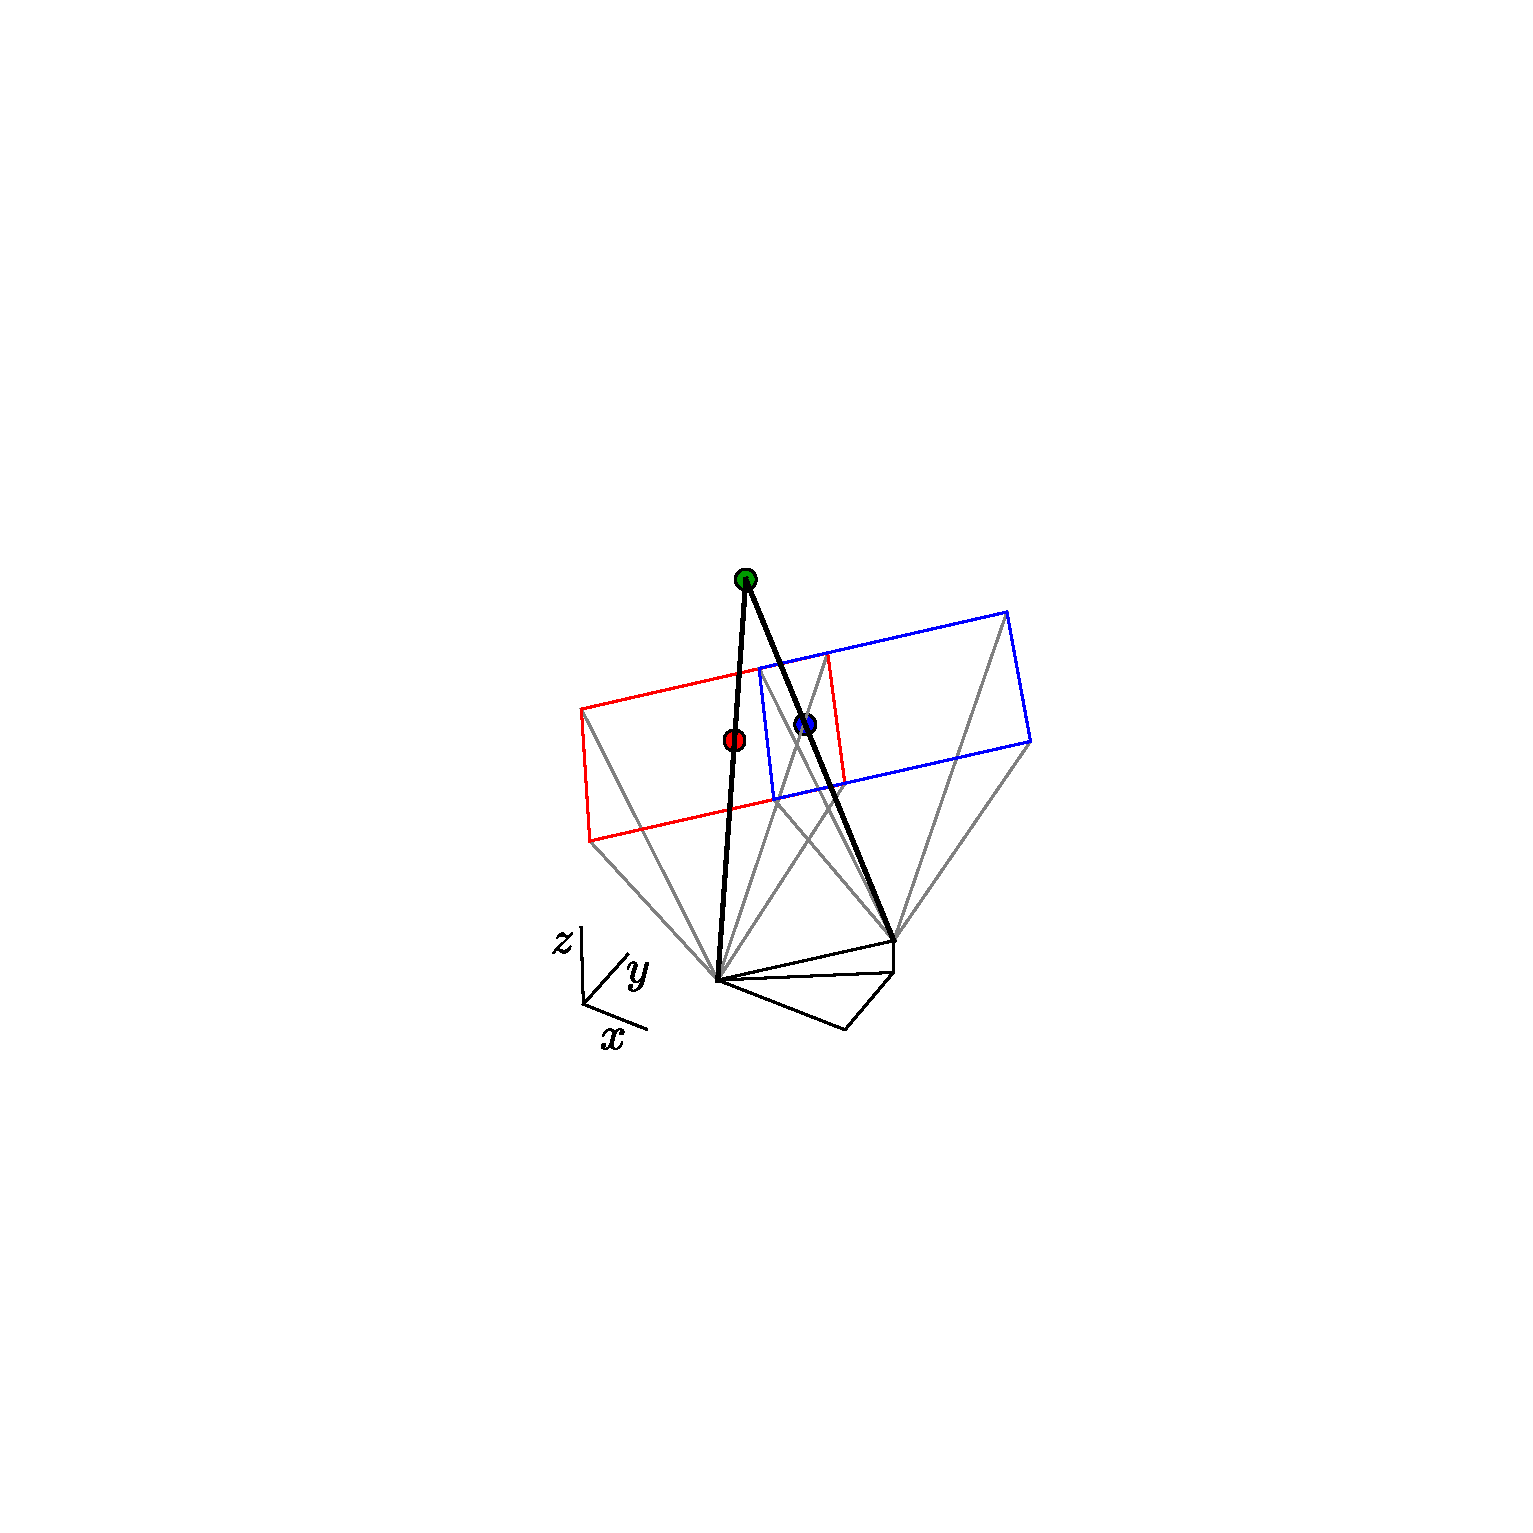
\includegraphics[clip,trim=9cm 7.7cm 8cm 9cm,height=5cm]{3dpoints}
\caption{Illustration of the computation of a point in 3D.}
\label{fig:3dpoints}
\end{figure}

Figure~\ref{fig:result-real-image} shows the resulting point cloud for an image pair from the  sequence. We distinguish two different clusters: the first is at an altitude of about $700$ meters and corresponds to the cumulus cloud at the bottom right of the input image, while the second represents the higher cloud layer appearing at around $3000$ meters.

\begin{figure}[htb]
\centering
\includegraphics[height=5.5cm]{result-3D}
\caption{3D point cloud computed for a pair of images from the sequence.}
\label{fig:result-real-image}
\end{figure}




\subsection{Validation}
Since it is very difficult to measure the actual 3D location and shape of clouds, we use computer-generated images with a user-defined cloud bottom altitude for validating our approach. We use \emph{Blender},\footnote{~\url{http://www.blender.org/}} an open-source 3D computer graphics program, for creating images using a procedural cloud shader and a model of the fish-eye lens of WAHRSIS. While being simpler than the reality, these images do have the advantage that the positions of the imagers and clouds can be user-defined. 

For this experiment, we created a sequence of $21$ frames with a cloud moving over the two cameras. The average cloud bottom altitude is $500$ meters, and the distance between the cameras is $400$ meters. Fig.~\ref{fig:blender-generated} shows an example of such an image pair.

\begin{figure}[htb]
\centering
\includegraphics[height=4cm]{blender1}
\includegraphics[height=4cm]{blender2}
\caption{Image pair from the computer-generated sequence.}
\label{fig:blender-generated}
\end{figure}

\begin{figure}[htb]
\centering
\subfloat[3D view]{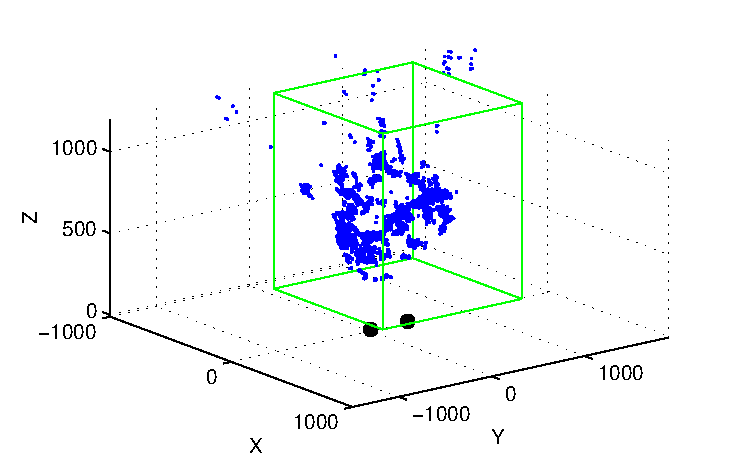
\includegraphics[height=3.6cm]{3D-generate}}
\subfloat[2D projection]{\includegraphics[height=3.6cm]{projection}}
\subfloat[Ground truth for (b)]{\includegraphics[height=3.6cm]{ground_truth}}
\caption[Illustration of 3D point cloud for an image pair computer from the computer-generated sequence.]{3D point cloud for an image pair computer from the computer-generated sequence.  The bounding boxes in which Blender generates the cloud are shown in green. The two black dots indicate the position of the imagers.}\label{fig:results-blender}
\end{figure}

Figure~\ref{fig:results-blender} shows the resulting 3D point cloud for an image pair from the computer-generated sequence. It matches with the ground truth created by Blender. Averaging over the entire sequence, 82.4\% of the reconstructed 3D points lie inside the bounding box in which the cloud is generated.


In this section, we have discussed how 3D scene flow techniques can be used to estimate cloud base height in a multiple-camera setting. We have introduced a workflow to a common scene flow algorithm in this context, which we validated with computer generated images. 


\section{Conclusion}
\label{sec:chap8-conclude}
In this chapter, we have proposed a point localization algorithm in a multiple-camera setting, under the assumption of error-free feature matching and noisy camera poses. Our modified SHARP algorithm has the best performance as compared to the other benchmarking algorithms. In the later part of this chapter, we demonstrate a practical example of point localization task---localizing cloud mass in the 3D space using a pair of ground-based sky cameras. Our theoretical analysis on point localization in multi-camera setup serves us an attempt to understand the accuracy of the cloud base height estimation. In practice, point localization in the 3D space is a challenging task, as it depends on a number of important factors: error-free feature matching and tracking, accurate estimation of camera poses and dense feature correspondence between stereo images. The task gets more challenging in cloud base height estimation, as clouds are generally featureless and feature matching between two images gets more challenging. 




































